\section{Panorama energetico attuale}
La \textit{rete elettrica} attuale è il risultato di una rapida urbanizzazione e di un rapido sviluppo di infrastrutture in varie zone del mondo. Sebbene tali reti esistano ormai in molte aree geografiche diverse, le aziende generalmente tendono ad adottare tecnologie molto simili tra di loro. Ciononostante, restano altri fattori  di varia natura (economica, politica, geografica) legati allo sviluppo energetico che si diversificano a seconda dell'azienda. \newline
In generale però, pur tenendo in considerazione le differenze portate da tali fattori, la topologia base della rete elettrica attuale è rimasta immutata.
\begin{figure}[h] \centering{
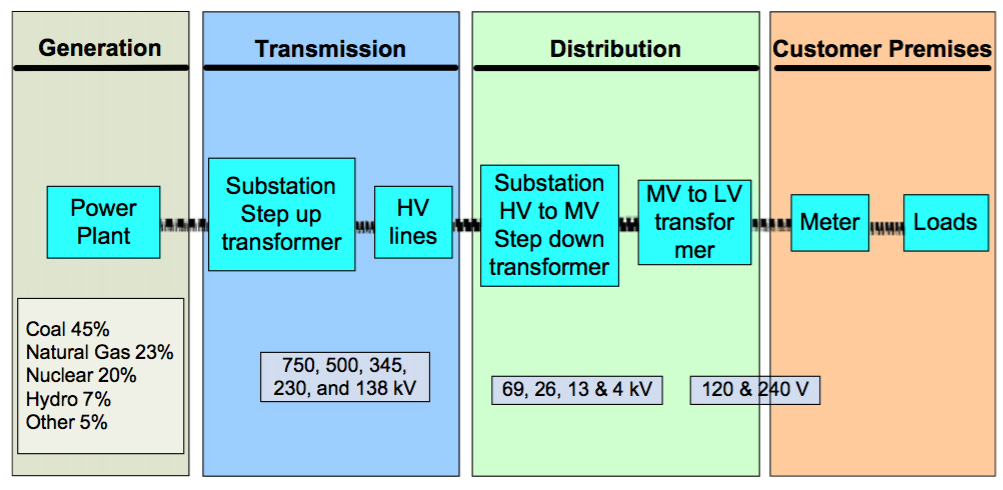
\includegraphics[scale=0.3, natwidth=1003,natheight=490]{imgs/elect_grid.png}}
\caption{La rete elettrica attuale}\label{fig:1}
\end{figure}
\newline La struttura della rete attuale è una struttura strettamente gerarchica. La figura \ref{fig:1} mostra l'esistenza di tre sottosistemi distinti: generazione, trasmissione e distribuzione \cite{pathsg}. \newline Le centrali elettriche sono composte da generatori elettromeccanici i quali, durante la fase di \textbf{generazione}, spinti dal flusso dell'acqua corrente o da motori termici alimentati da combustioni chimiche, generano energia. Tale energia viene successivamente inviata ai trasformatori del livello di \textbf{trasmissione}, i quali la convertiranno in energia ad alto voltaggio per permetterne la diffusione a lunga distanza. Dopo tale step, si passa alla \textbf{distribuzione}, in cui si applica prima una trasformazione a medio e basso voltaggio e, in seguito, si procede all'erogazione agli utenti finali.
\newline Tale sistema è basato sostanzialmente su una comunicazione \textit{unidirezionale} in cui la sorgente non ha nessuna informazione real-time circa le necessità degli ultimi punti della catena. Pertanto si tende a sovraccaricare la rete, facendole raggiungere a priori i picchi massimi di carico; poiché è raro che le richieste degli utenti raggiungano tali valori, questo approccio porta a rendere la rete elettrica un meccanismo inefficiente.
\newline
Inoltre, le reti elettriche attuali sono interconnesse tra loro a formare reti regionali o nazionali con lo scopo di fornire rotte ridondanti e alternative per il flusso della corrente in caso di problemi. \newline
La distribuzione dell'energia è gestita da un \textit{controllore centralizzato} che ha il compito di amministrare diverse regioni da un'unica posizione centrale. 

\section{Cenni storici}
Le tecnologie relative alle reti elettriche hanno radici che risalgono alla fine del XIX secolo: la \textit{corrente continua} di Thomas Edison e la \textit{corrente alternata} di Nikola Tesla continuano ad essere utilizzate tutt'ora. Oggi, infatti, l'energia viene trasmessa utilizzando la corrente alternata, mentre quella continua ha applicazioni specifiche, solitamente all'interno di plessi residenziali e commerciali. \newline \newline
In accordo a \cite{securingSG}, le principali topologie di rete elettrica attualmente in uso sono due: \textbf{radial grid} e \textbf{mesh grid}.


\begin{figure}[h]\centering{
  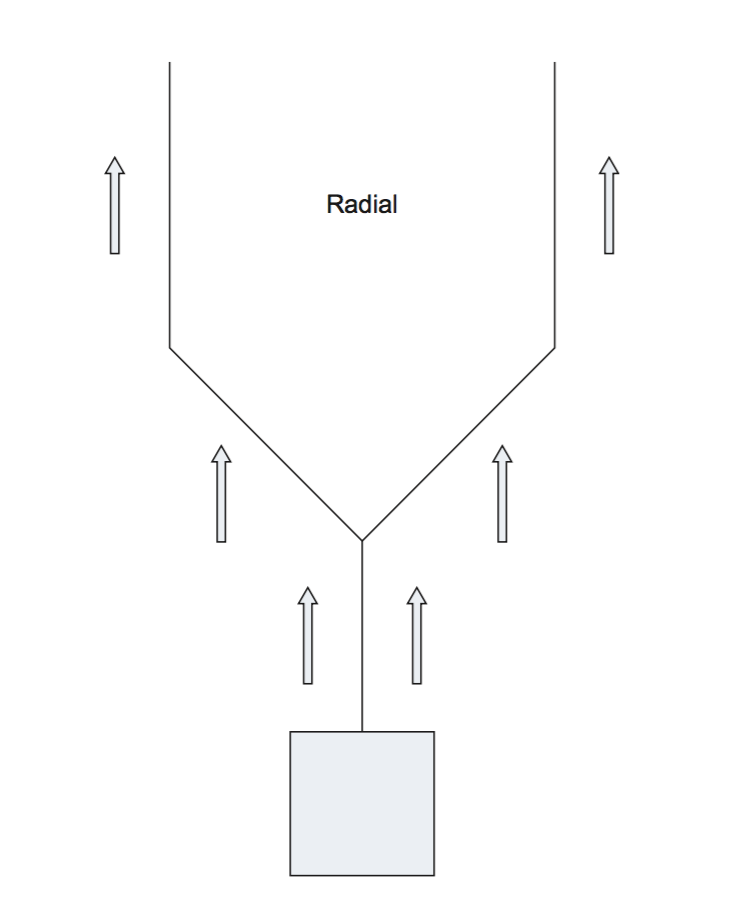
\includegraphics[scale=0.2, natwidth=754,natheight=909]{imgs/radialgrid.png}
  \caption{Radial grid}\label{fig:2}
}
\end{figure}

La radial grid (vedi Figura \ref{fig:2}) è la topologia più comune; in essa l'elettricità viene distribuita a partire da una sottostazione seguendo un modello che ricorda un albero con molti rami e foglie.
Man mano che l'energia fluisce attraverso i cavi elettrici, la sua forza viene ridotta finchè non raggiunge la destinazione.

\begin{figure}[h]\centering{
  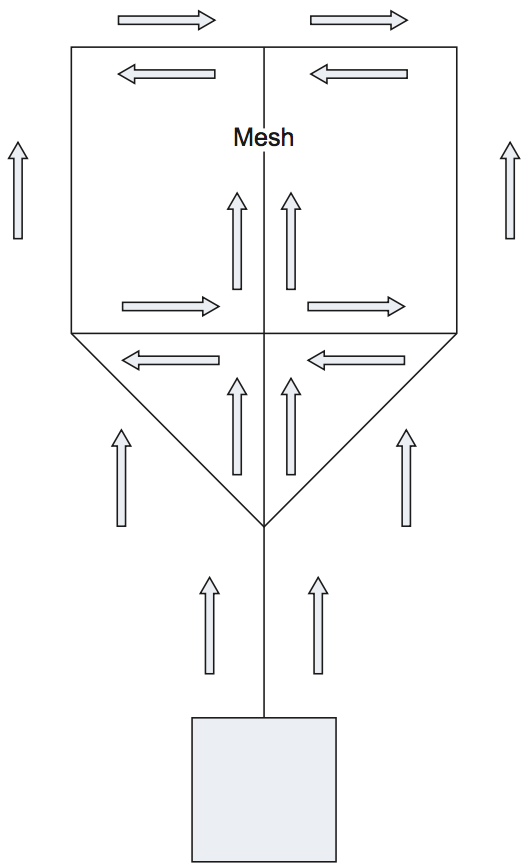
\includegraphics[scale=0.2, natwidth=529,natheight=867]{imgs/meshgrid.png}
  \caption{Mesh grid}\label{fig:3}
}
\end{figure}

La mesh grid (vedi Figura \ref{fig:3}) fornisce una maggiore affidabilità rispetto alla radial grid poichè in quest'ultima ogni ramo ed ogni foglia ricevono energia da una singola sorgente (l'albero), mentre in una mesh l'energia può essere fornita attraverso varie fonti (altri rami e foglie). \newline
Le radial grid forniscono, inoltre, ridondanza limitata: in caso di malfunzionamento, una sottostazione vicina può entrare a far parte della rete, ma ciò presuppone che tale sottostazione non sia nelle stesse condizioni di quella che ha generato il guasto. \newline
Queste due topologie sono molto diffuse negli Stati Uniti.
Vi è, poi, una terza topologia utilizzata principalmente in Europa: \textbf{looped topology}, nata come insieme delle due reti precedenti (vedi Figura \ref{fig:4}). 

\begin{figure}[h]\centering{
  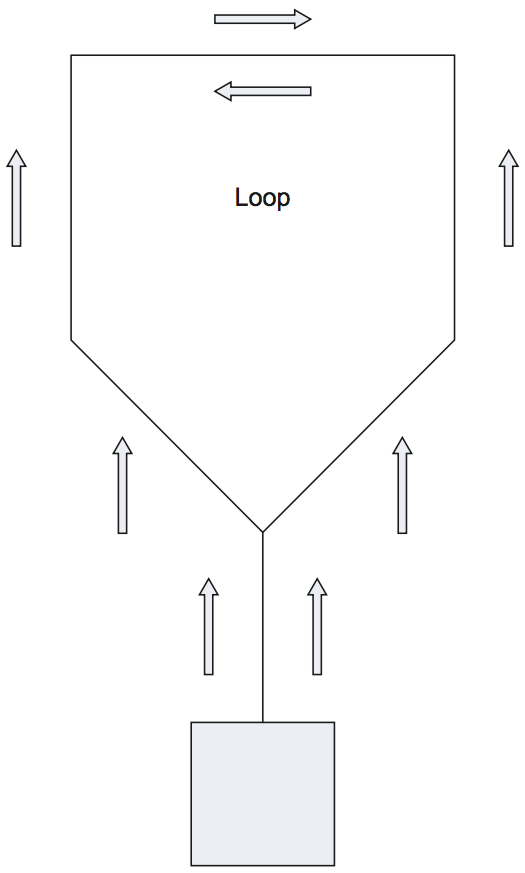
\includegraphics[scale=0.2, natwidth=525,natheight=873]{imgs/looptop.png}
  \caption{Looped topology}\label{fig:4}
}
\end{figure}
\newpage
Tale topologia è molto simile alla radial grid, ad eccezione del fatto che, a partire dalla sottostazione, i rami e le foglie hanno due cammini separati. L'obiettivo della looped topology è essere capace di resistere alle rotture interne alla rete, indipendentemente dal punto in cui si verificano; per questo motivo tale topologia risulta essere più costosa rispetto alla radial grid.
\newline \newline
Con il passare del tempo si è sentita sempre di più la necessità di svecchiare tali topologie, tenendo in conto tanti fattori e tante motivazioni.\newline
Considerando, per esempio, che quasi il 90\% dei guasti alla rete elettrica provengono dal sottosistema di distribuzione, le modifiche e i miglioramenti partono proprio da quest'ultimo. Inoltre, il rapido aumento dei costi relativi ai combustibili fossili insieme all'inabilità delle aziende di espandere la loro potenza di generazione mantenendola in linea con la domanda sempre più crescente, ha accelerato il bisogno di modernizzare la rete di distribuzione introducendo tecnologie capaci di gestire meglio sia le richieste che i guadagni ottenuti. \newline
\begin{figure}[h]\centering{
  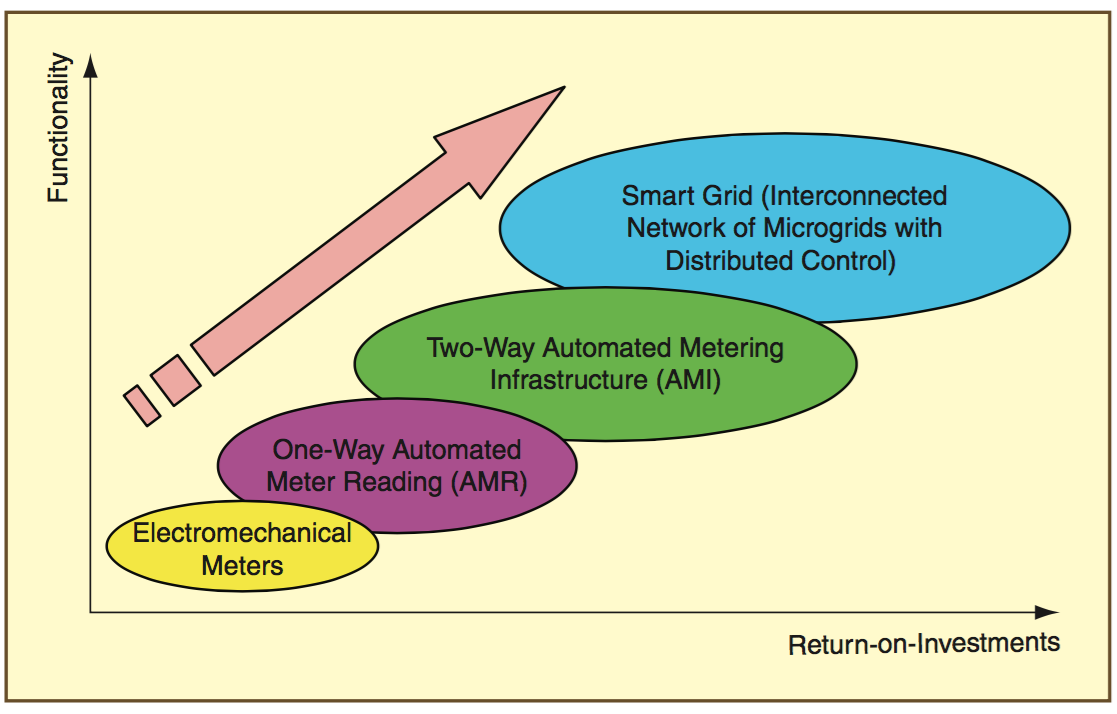
\includegraphics[scale=0.2, natwidth=1117,natheight=714]{imgs/evolution.png}
  \caption{L'evoluzione della smart grid}\label{fig:5}
}
\end{figure}

La Figura \ref{fig:5} mostra che gli investimenti degli ultimi anni si sono focalizzati principalmente sull'aspetto della rete elettrica che riguarda le misurazioni (\textit{metering}). \newline I primi progetti in questo settore hanno visto la nascita dei sistemi di \textbf{automated meter reading} (AMR) all'interno del sistema di distribuzione \cite{securingSG}. \newline
L'infrastruttura AMR, nata nel 1977, ha introdotto l'automazione nella rete elettrica. Attraverso una combinazione di tecnologie, incluse reti wireless e wired,   AMR ha permesso alle compagnie di leggere le misurazioni da remoto, di ottenere le informazioni quasi in real-time e di fornire agli utenti bollette basate sui loro consumi reali (in precedenza le compagnie emettevano le bollette basandosi sulle stime dei consumi del cliente).  \newline Inoltre, grazie a questo meccanismo di recupero informazioni tempestivo, le aziende sono state capaci di migliorare la produzione di energia attraverso un maggiore controllo durante periodi di alta e bassa richiesta. \newline \newline
Sebbene la teconologia AMR all'inizio abbia attirato molta attenzione, le aziende presto si sono rese conto che non risolve il loro problema principale: la gestione demand-side. A causa della sua comunicazione unidirezionale, le capacità di AMR sono ridotte alla sola lettura dei dati e non è permesso, per esempio, modificare il comportamento della rete a seconda delle informazioni ricevute. \newline Pertanto AMR ha avuto vita breve; le aziende, piuttosto che continuare ad investire su di essa, hanno preferito spostarsi verso l'\textbf{advanced metering infrastructure} (AMI). \newline
L'AMI (di cui si parlerà in dettaglio nel Capitolo 3), è un'architettura che permette la comunicazione automatizzata e bidirezionale tra uno smart meter e una società di servizi. L'obiettivo è quello di fornire a tali società informazioni real-time circa i consumi energetici e permettere agli utenti di fare scelte consapevoli sull'utilizzo dell'energia basate sui costi all'istante di utilizzo.
\newline
\newline
Il passo successivo nell'evoluzione della distribuzione della corrente elettrica è costituito dalla \textbf{Smart Grid}, che utilizza l'AMI come componente core per il recupero delle informazioni circa lo stato della rete e i consumi utente.


\section{Perché la Smart Grid?}
Le industrie del settore dei servizi pubblici di tutto il mondo attualmente cercano di risolvere numerosi problemi, tra cui 
\begin{itemize}
\item Diversificazione della generazione di energia;
\item Gestione delle richieste utente;
\item Conservazione dell'energia;
\item Riduzione globale dell'emissione di anidride carbonica.
\end{itemize}
È evidente che tali problemi non possono essere risolti facendo affidamento sulla rete elettrica esistente. \newline
Come detto in precedenza, la natura della comunicazione della rete attuale è unidirezionale. Essa, inoltre, converte solo un terzo di energia in elettricità, senza preoccuparsi del calore disperso. Circa l'8\% della corrente prodotta, viene dissipata poi attraverso i cavi elettrici, mentre il 20\% viene riservata ad eventuali picchi di carico di richieste utente (ed è in uso solo il 5\% delle volte). \newline
In aggiunta a tali problemi, vi è l'inadeguatezza della struttura gerarchica della rete. A causa di tale organizzazione, infatti, si ha un \textit{effetto domino dei guasti}, in cui un fallimento verificatosi all'interno di uno dei tre sottosistemi può influire significativamente sugli altri. \newline
La rete elettrica di nuova generazione, la Smart Grid, si propone di occuparsi delle maggiori carenze della rete attuale.
\begin{figure}[h]\centering{
  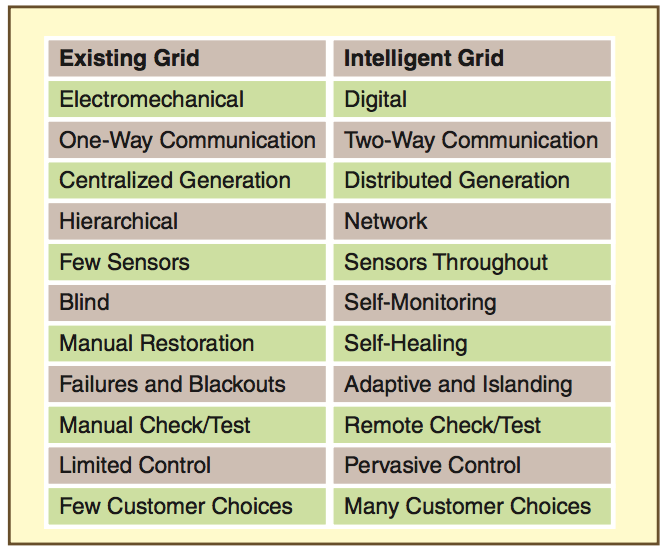
\includegraphics[scale=0.3, natwidth=669,natheight=553]{imgs/differences.png}
  \caption{Differenze tra la rete elettrica attuale e la Smart Grid}\label{fig:6}
}
\end{figure}

A partire dal 2005, c'è stato un interesse sempre più crescente verso le Smart Grid. Il riconoscere che l'ICT (\textit{Information and Communication Technology}) offre significative opportunità per modernizzare il funzionamento delle reti elettriche unito alla consapevolezza che la produzione di energia può essere migliorata solo con un continuo ed efficiente monitoraggio, ha fatto sì che si muovessero i primi passi verso la Smart Grid. In aggiunta a tali fattori, ci sono anche altre motivazioni a favore del passaggio verso una rete elettrica moderna \cite{smartgrid}:
\begin{itemize}
\item \textit{Strutture non più adeguate}: in molte zone del mondo (per esempio in USA e in alcuni paesi dell'Europa), i sistemi si sono rapidamente espansi a partire dal 1950; le strutture relative alla trasmissione e alla distribuzione che furono installate a quel tempo non sono più adatte e devono essere sostituite. Il bisogno di rinnovare tali componenti è un'ovvia opportunità di innovazione e, quindi, di introduzione di nuovi modelli e pratiche operative. A ciò si aggiunge il fatto che, in molti paesi, i circuiti elettrici hanno bisogno di adattarsi ai carichi sempre più crescenti e all'introduzione di nuove fonti di energia rinnovabili. Ciò richiede, quindi, metodi più intelligenti sia per aumentare la capacità di trasmissione dell'energia, sia per reindirizzare il flusso di corrente verso circuiti meno carichi;

\item \textit{Vincoli termici}: si riferiscono ai limiti dei sistemi di trasmissione e distribuzione relativamente alla loro capacità di diffusione dell'energia. Quando le attrezzature trasportano la corrente eccedendo la loro potenza termica, si surriscaldano e i materiali atti all'isolamento si deteriorano rapidamente. Ciò comporta una riduzione della vita delle attrezzature e un aumento di possibilità di fallimenti.\newline I vincoli termici dipendono molto dalle condizioni dell'ambiente esterno, che cambiano durante gli anni. Pertanto l'uso di rate di trasmissione e distribuzione dinamici può aumentare la capacità del circuito;



\item \textit{Vincoli operativi}: qualsiasi sistema opera all'interno di predefiniti vincoli di voltaggio e frequenza. Se il voltaggio eccede il limite, i materiali isolanti dei componenti del sistema e le attrezzature degli utenti possono essere danneggiate e causare corto-circuito. \newline Per quanto riguarda la frequenza invece, si tende a mantenerla all'interno di un range molto piccolo e, quando varia, intervengono dei servizi appositi che hanno il compito di riportarla nell'intervallo prestabilito. \newline
La generazione di energia rinnovabile, però, ha un output variabile che non può essere previsto con certezza in anticipo. Pertanto mantenere il bilancio erogazione-richiesta e la frequenza del sistema nei limiti risulta essere un compito arduo. Per tale motivo si è sempre alla ricerca di nuovi servizi per la gestione della frequenza. \newline Si pensa che in futuro l'utilizzo delle Smart Grid in vari ambiti, per esempio domestico e automobilistico, porterà ad avere carichi sempre più flessibili; ciò aiuterà nel mantenere la stabilità della rete;

\item \textit{Sicurezza delle forniture}: la società moderna richiede che la fornitura di energia sia sempre più affidabile, man mano che carichi sempre più critici vengono connessi alla rete. L'approccio tradizionale per migliorare l'affidabilità, come visto in precedenza, era quello di installare cammini ridondanti, con notevole impatto sia sui costi che sull'ambiente. \newline L'approccio della Smart Grid in caso di guasti, invece, prevede l'utilizzo di intelligenti meccanismi di riconfigurazione, in modo tale da mantenere costante la fornitura ai clienti ma evitando i costi addizionali portati da ulteriori circuiti;
\item \textit{Iniziative nazionali}: molti governi nazionali incoraggiano le iniziative delle Smart Grid poiché le considerano un meccanismo redditizio ma, allo stesso tempo, economico per rinnovare le loro infrastrutture e introdurre risorse rinnovabili.
\end{itemize}

\begin{figure}[h]\centering{
  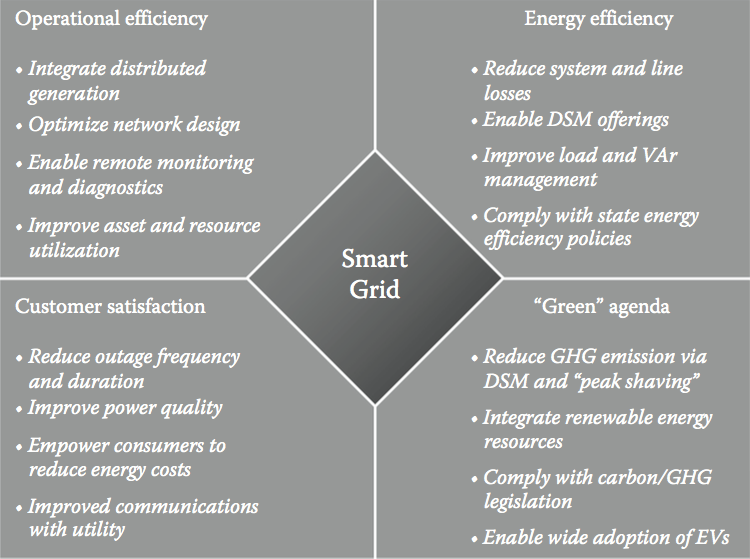
\includegraphics[scale=0.3, natwidth=750,natheight=559]{imgs/benefits.png}
  \caption{Benefici introdotti dalla Smart Grid}\label{fig:7}
}
\end{figure}

La figura \ref{fig:7} mostra i vantaggi introdotti dall'utilizzo delle Smart Grid. Lo sviluppo di tale rete moderna non dovrebbe essere basato solo su ``soluzioni abilitanti", ma anche su ``soluzioni integrate" che rispondano ai problemi operativi e aziendali e che forniscano benefici significativi, misurabili e durevoli agli utenti, al servizio pubblico, all'economia e all'ambiente.
\newline 
Di estrema importanza nell'implementazione delle soluzioni proposte dalla Smart Grid sono i seguenti aspetti:
\begin{itemize}
\item Migliorare l'affidabilità dell'energia dei servizi pubblici, le performance operative e la produttività generale;
\item Aumentare l'efficienza energetica e diminuire le emissioni di anidride carbonica;
\item Permettere agli utenti di gestire i loro consumi energetici risparmiando energia ma, allo stesso tempo, senza modificare il loro stile di vita;
\item Ottimizzare l'integrazione di energie rinnovabili.
\end{itemize}

\section{Cos'è la Smart Grid?}
Il concetto di Smart Grid mette insieme una serie di tecnologie e soluzioni per gli utenti finali e affronta, inoltre, concetti politici e normativi. \newline Non esiste una singola definizione chiara e precisa; in  \cite{smartgrid} è possibile trovare una serie di caratterizzazioni. \newline L'European Technology Platform definisce la Smart Grid nel seguente modo:
\begin{quote}
\textit{``Una Smart Grid è una rete elettrica che può integrare intelligentemente le azioni di tutti gli utenti connesse ad essa - generatori, consumatori - in modo da fornire efficientemente un'alimentazione elettrica che sia sostenibile, economica e sicura."}
\end{quote}
In accordo all'US Department of Energy:
\begin{quote}
\textit{``Una Smart Grid utilizza la tecnologia digitale per migliorare l'affidabilità, la sicurezza e l'efficienza (sia economica che energetica) del sistema elettrico, a partire dalla generazione su larga scala, attraverso il sistema di distribuzione, fino ai consumatori, ed attraverso un numero crescente di risorse di storage e  di generazione distribuita."}
\end{quote}
Secondo 	\emph{Smarter Grids: The Opportunity}, invece, la Smart Grid è definita come:
\begin{quote}
\textit{``Una Smart Grid utilizza sensing, embedded processing e comunicazioni digitali per far sì che la rete elettrica sia osservabile (capace di essere misurata e visualizzata), controllabile (capace di essere manipolata ed utilizzata), automatizzata (capace di adattarsi ed autoripararsi), pienamente integrata (pienamente interoperabile con sistemi esistenti e con la capcità di incorporare un insieme di diverse sorgenti energetiche)."}
\end{quote}
\cite{smartgrid} suggerisce, inoltre, i seguenti attributi per una Smart Grid:
\begin{itemize}
\item Permette la gestione ``demand side" sia attraverso l'integrazione di smart meter, elettrodomestici intelligenti, micro-generazione e conservazione dell'energia sia fornendo agli utenti informazioni circa i loro utilizzi e i prezzi;
\item Facilita l'introduzione di fonti di energia rinnovabile e di generazione distribuita, riducendo così l'impatto ambientale dell'intero settore energetico; 
\item Assicura e migliora l'affidabilità e la sicurezza delle forniture, resistendo agli attacchi, ai disturbi e ai disastri naturali, anticipando e affrontando i problemi del sistema e migliorando le funzionalità di trasferimento dell'energia;
\item Mantiene alta la qualità della fornitura di energia elettrica per soddisfare le apparecchiature sempre più sofisticate che aumentano con l'economia digitale.
\end{itemize}
\begin{figure}[h]\centering{
  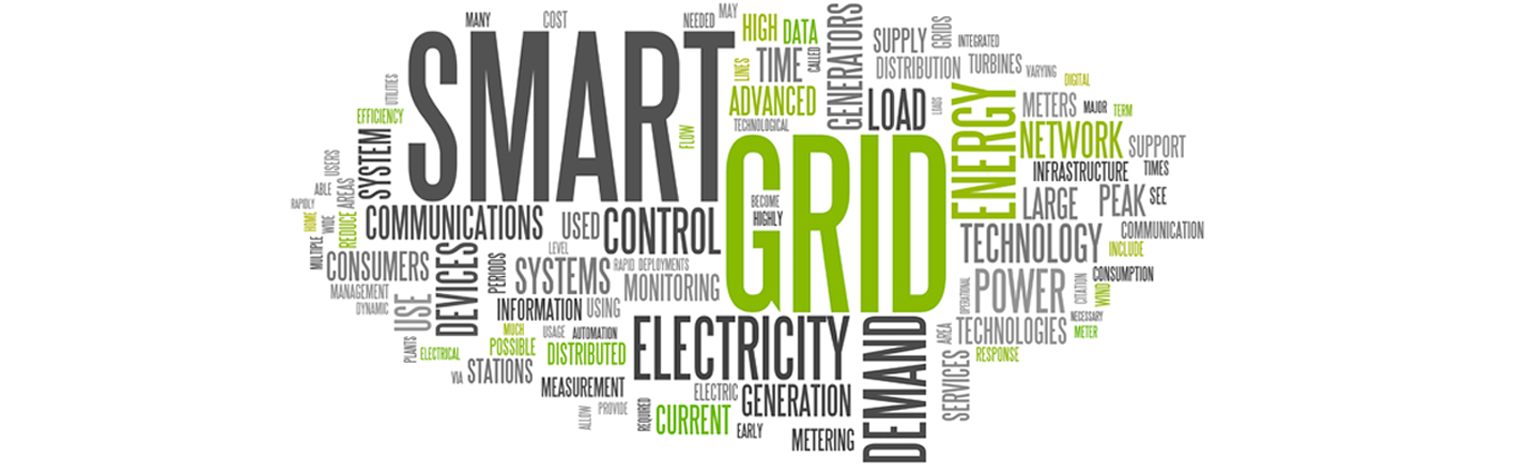
\includegraphics[scale=0.25, natwidth=1522,natheight=466]{imgs/wordcloud.png}
}
\end{figure}
\section{Requisiti di una Smart Grid}
Monitoraggio/\emph{sensing}, comunicazione e controllo sono i tre \emph{building block} fondamentali che convertono un sistema di distribuzione di energia in una Smart Grid. Le componenti di monitoraggio/sensing devono essere capaci di rilevare malfunzionamenti o deviazioni dal normale range operativo della rete elettrica. Inoltre, poichè in una Smart Grid un punto di consumo elettrico può diventare anche un punto di generazione, il processo di sensing deve essere strettamente collegato al processo di \emph{metering}. \newline
I sistemi di comunicazione devono permettere che l'input dei sensori raggiunga gli elementi di controllo della Smart Grid, i quali genereranno dei messaggi con il compito di assicurarsi che la trasmissione nei vari punti della rete sia conforme alle aspettative. Ci sono, inoltre, altri requisiti importanti per le infrastrutture di comunicazione, di cui si discutono i dettagli nel resto di questo paragrafo \cite{surveymotiv}.
\newline \newline
\textit{Quality of Service:} è necessario garantire la \emph{QoS} per le tecnologie di comunicazione e di rete utilizzate all'interno della Smart Grid, partendo dalla generazione dell'energia, passando per trasmissione e distribuzione e finendo alle applicazioni utente. In particolare, ci si focalizza su due parametri: \emph{latenza} e \emph{larghezza di banda}.\newline
Per quanto riguarda la latenza, la comunicazione in una Smart Grid è caratterizzata dal fatto che la maggior parte delle interazioni devono avvenire in tempo reale. Per scopi di sensing/misurazione, i messaggi di lettura dovrebbero essere trasmessi all'interno di un \emph{frame temporale} molto piccolo. Per esempio, il tempo massimo di trasmissione ammesso è nel range dei 12-20 ms. I valori misurati non dovrebbero essere generati da più di 15 secondi quando arrivano al centro di controllo. \newline
Per quanto riguarda la larghezza di banda, durante l'evoluzione di una Smart Grid, mediante l'aggiunta ad essa di elementi sempre più intelligenti, l'infrastruttura di comunicazione dovrebbe essere capace di trasmettere un numero sempre più crescente di messaggi simultaneamente, senza grave impatto sulla latenza. La banda di rete deve aumentare più rapidamente rispetto alla richiesta di tali elementi intelligenti nella rete.
\newline \newline
\textit{Interoperabilità:} si riferisce all'abilità delle diverse parti di una Smart Grid di lavorare insieme, di utilizzare componenti compatibili, di scambiarsi informazioni tra di loro e lavorare in maniera cooperativa per completare i task. Tale requisito rende effettiva l'integrazione e la comunicazione bidirezionale tra i tanti elementi interconnessi della rete.\newline
Il \emph{NIST} ha sviluppato un framework che include protocolli e standard per la gestione delle informazioni, in modo da raggiungere l'interoperabilità tra i dispositivi della Smart Grid e i sistemi. Maggiori dettagli in \cite{surveymotiv}.
\newline \newline
\textit{Scalabilità:} è necessaria per facilitare l'inserimento all'interno della Smart Grid sia di tanti nuovi dispositivi e servizi, che di tanti meccanismi di monitoraggio real-time dell'interazione dell'utente finale. \newline
\cite{surveymotiv} propone una rete \emph{IP-based} come soluzione efficace per i bisogni dell'infrastruttura di comunicazione.
\newline \newline
\textit{Sicurezza:} in accordo all'\emph{Electric Power Research Institute (EPRI)}, uno dei requisiti emergenti dello sviluppo delle Smart Grid è relato alla \textbf{cyber security} dei sistemi. Come indicato nel loro report \cite{surveymotiv}, la sicurezza informatica del sistema di comunicazione è un problema critico, a causa dell'aumento del potenziale degli attacchi e degli incidenti che si verificano in esso. \newline 
La cyber security deve occuparsi non solo di attacchi deliberati, come quelli provenienti, ad esempio, da dipendenti non contenti, da spionaggio industriale e da terroristi, ma anche di manomissioni involontarie dell'infrastruttura di informazione dovute ad errori degli utenti, fallimenti delle attrezzature e disastri naturali. Le vulnerabilità potrebbero permettere, infatti, ad un attaccante di penetrare nella rete, ottenere accesso al software di controllo e alterare le condizioni di carico per destabilizzare la rete. \newline
Attualmente, molte organizzazioni lavorano sullo sviluppo dei requisiti di sicurezza nella Smart Grid, tra cui North American Electrical Reliability Corporation-Critical Infrastructure Protection (NERC-CIP), IEEE, National Infrastructure Protection Plan (NIPP), e NIST. \newline 
Denominatore comune di tutti gli standard in via di sviluppo è il seguente concetto: la sicurezza delle comunicazioni nella Smart Grid dipenderà fortemente da autenticazione, autorizzazione e tecnologie per la \emph{privacy}. \newline Tutte le tecnologie sviluppate, poggiano su una sorta di gestione della chiave. Considerando il fatto che la Smart Grid conterrà milioni di dispositivi, diffusi tra tante organizzazioni, i sistemi di gestione della chiave utilizzati dovranno essere altamente scalabili e garantire i livelli massimi possibili di efficienza.
\newline \newline
\textit{Standardizzazione:} la Smart Grid coinvolge al suo interno una serie di standard come, ad esempio, nella generazione dell'energia, nella distribuzione e nel controllo oltre che nella comunicazione. IEEE recentemente ha preso l'iniziativa per definire questi standard e linee guida su come la Smart Grid dovrebbe operare utilizzando le ultime tecnologie nell'ingegnerizzazione dell'energia, controllo, comunicazione e informazione; il gruppo che è stato creato prende il nome di IEEE P2030 group \cite{surveymotiv}. \newline Per quanto riguarda l'ingegnerizzazione dell'energia, ci si focalizza sui requisiti di interoperabilità. Per quanto riguarda l'informazione, invece, si affrontano problemi relativi alla privacy, sicurezza, integrità dei dati, interoperabilità e interfacce. Per la comunicazione, infine, si definiscono i requisiti per l'interazione tra i dispositivi e si stabiliscono limiti per generazione, distribuzione e trasmissione in collaborazione con i clienti.
 

\section{Tecnologie coinvolte}
Per soddisfare tutti i requisiti della Smart Grid, è necessario sviluppare ed implementare le seguenti tecnologie \cite{smartgrid}:
\begin{enumerate}
\item \textit{Tecnologie per l'informazione e la comunicazione}, che includono
	\begin{itemize}
	\item Meccanismi per la comunicazione bidirezionale tra le varie componenti del sistema;
	\item Architetture aperte per il collegamento e l'utilizzo semplice di elettrodomestici e veicoli elettrici;
	\item Componenti hardware e software necessari per fornire ai clienti sempre più informazioni;
	\item Software per garantire la sicurezza delle informazioni e standard per fornire scalabilità e interoperabilità tra i sistemi di informazione e comunicazione.
	\end{itemize} 
\item \textit{Tecnologie per misurazioni, sensing, controllo ed automazione}, che includono
	\begin{itemize}
	\item \textit{Intelligent Electronic Devices} (IED) per fornire inoltro, misurazioni e memorizzazione di fallimenti ed eventi per il sistema energetico in maniera avanzata;
	\item \textit{Phasor Measurement Units} (PMU) e \textit{Wide Area Monitoring, Protection and Control} (WAMPAC) per garantire la sicurezza del sistema;
	\item Sistemi integrati di sensing, misurazione, controllo ed automazione e tecnologie per l'informazione e la comunicazione per fornire rapide diagnosi e risposte tempestive a qualsiasi evento in qualsiasi parte della rete;
	\item Elettrodomestici, comunicazione, controllo e monitoraggio più intelligenti per massimizzare la sicurezza, il comfort e il risparmio energetico delle abitazioni;
	\item Smart meter e tutti i software che permettano ai clienti di avere una maggiore scelta e un maggiore controllo sull'utilizzo di elettricità e gas. Tali meccanismi permetteranno, inoltre, di fornire ai clienti bollette più accurate e informazioni real-time più precise sui loro consumi.
	\end{itemize}
\item \textit{Tecnologie per la conservazione dell'energia}, che includono
	\begin{itemize}
	\item \textit{High Voltage Direct Current} (HVDC) e \textit{Flexible Alternate Current Transmission Systems} (FACTS) per abilitare le trasmissioni a lungo raggio e l'integrazione delle energie rinnovabili;
	\item Differenti interfacce e differenti dispositivi per fornire una connessione efficiente delle risorse rinnovabili e dei dispositivi per la conservazione dell'energia;
	\item Dispositivi per fornire un maggiore controllo sui flussi di energia nella rete a corrente alternata;
	\item  HDVC e FACTS in unione ad altri filtri, integrati nei meccanismi di comunicazione e controllo per assicurare una maggiore affidabilità e flessibilità del sistema e una migliore qualità dell'energia.
	\end{itemize}
\end{enumerate}